%!TEX root = ../report.tex

% 
% Related work
% 


\section{A State of the Art in Frameworks for Information Technology Governance and Management}

% Example citation:
In this section we will present a set of literature references on the subjects related to this project. We will present the most important frameworks on Information Systems Management and Governance with the objective of coming up with a choice of a framework or a set of them to implement our processes for project and maintenance management.\par
Our choice is centered in three frameworks we consider the most relevant for this project: COBIT 5, ITIL V3 and PMBOK. This three frameworks provide, from different perspectives, guides and principles for IT Governance and Management, presenting processes for achieving a successful implementation of this principles in an organization.

\subsection{IT Governance and IT Management}

One important concept to define is the difference between IT Governance and IT management. They are many times confused and some authors already tried to explain the difference between the two concepts.\par
Considering the definition given in \cite{ITGovAndMech}, \textit{``IT Management is focused on the internal effective supply of IT services and products and the management of present IT operations. IT Governance in turn is much broader, and concentrates on performing and transforming IT to meet present and future demands of the business (internal focus) and the business' customers (external focus).''}.\par
 Considering the COBIT 5 view for this question \cite{2012cobit}, there is a \textit{``clear distinction between governance and management, in the way these two disciplines encompass different types of activities, require different organizational structures and serve different purposes. Governance ensures that stakeholders' needs, conditions and options are evaluated to determine balanced, agreed-on enterprise objectives to be achieved. it sets direction through prioritisation and decision making and monitors performance and compliance against agreed-on direction and objectives.On the other hand, management plans, builds, runs and monitors activities in alignment with the direction set by the governance body to achieve the enterprise objectives.''}\par


 Considering both definitions, we can conclude that IT Governance has a bigger dimension that IT Management, but both need to be related and complementary to achieve success inside an organization. It is not possible for an organization to have well defined and matured management processes that are no related to governance aspects, but governance needs management to achieve goals and objectives settled to achieve success.

\subsection{COBIT 5}

Control Objectives for Information and Related Technology (COBIT) is a framework created by the Information Systems Audit and Control Association (ISACA) for IT Management and IT Governance.\par
As stated by ISACA \cite{2012cobit},\textit{``COBIT 5 provides a comprehensive framework that assists enterprises in achieving their objectives for the governance and management of enterprise IT. Simply stated, it helps enterprises create optimal value from IT by maintaining a balance between realizing benefits and optimizing risk levels and resource use''}. The framework is built on five basic principles:

\begin{itemize}
  \item Meeting the Stakeholders Needs 
  \item Covering the Enterprise End-to-end
  \item Applying a Single, Integrated Framework
  \item Enabling a Holistic Approach
  \item Separating Governance from Management
\end{itemize}


It also defines seven enablers, explained by COBIT as factors that, individually and collectively, influence whether governance and management over enterprise will work or not. This enablers can be categorized as:

\begin{itemize}
  \item Principles, Policies and frameworks 
  \item Processes 
  \item Organizational structures
  \item Culture, ethics and behavior 
  \item Information
  \item Services, infrastructure and applications
  \item People, skills and competencies
\end{itemize}

\begin{figure}
\centering
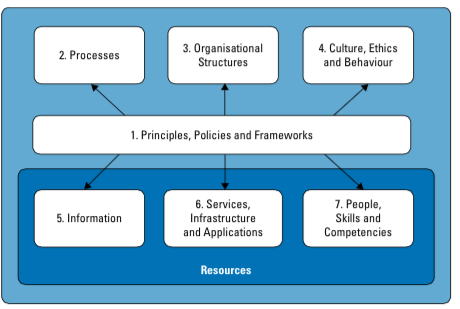
\includegraphics[width=0.5\textwidth]{img/Enablers.png}
\caption{COBIT 5 enablers. Extracted from \cite{2012cobit}.}
\end{figure}

Figure 2 presents the COBIT 5 enablers previous defined and how they relate among themselves in terms of its importance for the organization. Each enabler has stakeholders, a set of goals, a life cycle and can be defined good practices for each one.\par

\begin{figure}
\centering
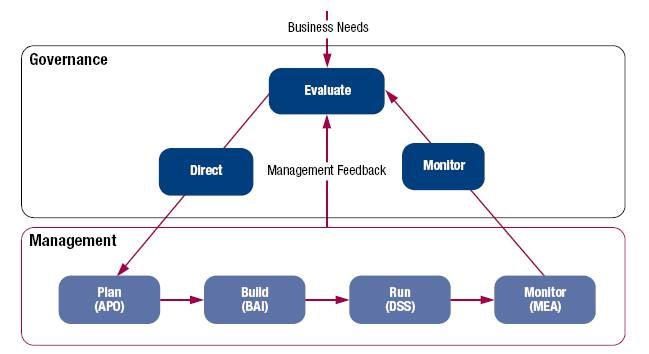
\includegraphics[width=0.7\textwidth]{img/COBITProcesses.jpg}
\caption{COBIT 5 domains. Extracted from \cite{2012cobit}.}
\end{figure}

Considering figure 3, COBIT 5 process reference model considers two big domains of processes: Governance and Management. The governance domain contains five processes in the domain Evaluate, Direct and Monitor(EDM). The management domain has four internal domains of processes: Align, Plan and Organise(APO), Build, Acquire and Implement(BAI), Deliver, Service and Support (DSS) and Monitor, Evaluate and Assess(MEA).\par
All processes for management and governance are presented in the Appendix B and all the implementation details explained in COBIT 5: Enabling Processes\cite{2012cobitEP}, a detailed reference guide to the processes defined in the COBIT 5 process reference model. This includes the COBIT 5 goals cascade, a process model explanation, governance and management practices, and the process reference model.\par
Relating to other frameworks and standards, COBIT tries to establish a framework that is compliant with the most widely accepted standards in IT governance and management. In figure 4 we can see the standards COBIT 5 relates by processes domain, with special attention to ITIL V3\cite{itilSS,itilSD,itilSO,itilST,itilCSI}, ISO/IEC 20000\cite{ISO20000-1}, PMBOK\cite{pmbok5} and CMMI\cite{cmmi}, that are closely related to this project's problem. This compliance with other standards is fundamental for a widely adoption of COBIT 5, in the way it tries to establish goals, metrics, practices, roles, inputs and outputs for each process, making it necessary being compliant with international standards. This will improve COBIT application and acceptance on organizations.\par

\begin{figure}[h!]
\centering
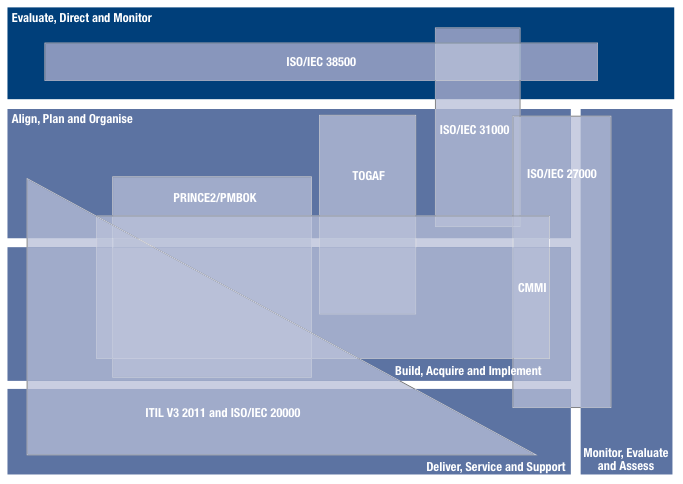
\includegraphics[width=0.7\textwidth]{img/COBITOtherFrameworks.png}
\caption{COBIT 5 coverage on other frameworks. Extracted from \cite{2012cobit}.}
\end{figure}


\subsubsection{CMMI}


CMMI (Capability Maturity Model Integration), first developed at the Software Engineering Institute at Carnegie Mellon University and currently operated by the CMMI Institute, consists on a set of practices and process improvement goals that organizations can use to evaluate and improve its processes. The CMMI framework provides all structures to produce models, training and appraisal methods.
Currently on version 1.3, it defines areas of interest that group collections of CMMI components for models, training and appraisal construction. The three areas of interest are:

\begin{itemize}

\item \textbf{CMMI for Acquisition (CMMI-ACQ)\cite{cmmiAcquisition}} - Provides guidance to organizations that manage the supply chain to acquire and integrate products and services to meet the needs of the customer.

\item \textbf{CMMI for Development (CMMI-DEV)\cite{cmmi}} - Provides guidance to improve the effectiveness, efficiency, and quality of their product development work. Used for process improvement in organizations that develop products.

\item \textbf{CMMI for Services (CMMI-SVC)\cite{cmmiServices}} - Provides guidance to organizations that establish, manage, and deliver services that meet the needs of customers and end users.

\end{itemize}

For this areas of interest, CMMI defines 16 core process areas, covering processes that are fundamental to improve the organization's processes. Each one of the areas is a set of related practices that, when implemented, will achieve goals important for process improvement.\par
CMMI supports two types of improvement paths, depending on the organization objectives. One is used for the organization to improve processes related to a specific process area, named the continuous representation, and the other one is used for organizations to improve a set of relating processes by incrementally consider sets of process areas, named the staged representation. As stated by CMMI, the continuous representation will allow to achieve capability levels and the staged representation will achieve maturity levels.\par
For the staged representation, the following capability levels are defined:

\begin{itemize}

\item \textbf{Level 0 - Incomplete} - Process not performed or only partially performed. Specific goals of process area not achieved.

\item \textbf{Level 1 - Performed} - Process performs the needed work to produce work products and satisfies the specific goals of the process area.

\item \textbf{Level 2 - Managed} - Performed process that is planned and executed according with policy.

\item \textbf{Level 3 - Defined} - Managed process that is tailored from the organization's set of standard processes according to the organization's tailoring guidelines.
 
\end{itemize}

For the continuous representation, the maturity levels defined are:

\begin{itemize}

\item \textbf{Level 1 - Initial} - Chaotic and Ad-Hoc processes. Organization does not provide a stable environment to support processes. Organizations are characterized by easily abandoning its processes and being unable to repeat them.

\item \textbf{Level 2 - Managed} - Projects establish the foundation for an organization to become an effective acquirer of needed capabilities by institutionalizing select project management and acquisition engineering processes. Processes, projects, products and services are managed and periodically evaluated. Processes are maintained in times of crisis.

\item \textbf{Level 3 - Defined} - Acquirers use defined processes for managing projects and suppliers. Project management and acquisition practices are embedded in the standard process set. Organization set of standards is established and improved over time. Processes described more rigorously than in level 2.

\item \textbf{Level 4 - Quantitatively Managed} - Acquirers establish quantitative objectives for quality and process performance and use them as criteria in managing processes. Process performance becomes predictable, controlled using statistical and quantitative techniques for prediction.

\item \textbf{Level 5 - Optimizing} - Process performance continuous improvement based on the organizations' objectives and performance needs comprehension. optimization is achieved through incremental and innovative process and technological improvements.

\end{itemize}

CMMI does not provide certification to organizations. Instead, it can be used to conduct appraisals, measuring the organization progress and earning maturity or capability levels face to CMMI Levels. These appraisals can be used for comparing the current practices with the CMMI best practices, finding areas to improve, for outside accreditation by suppliers and other stakeholders of conformance to a specific level of CMMI and to meets contractual requirements.\par
To conduct an CMMI appraisal, the organization must follow the appraisal Requirements for CMMI document \cite{appraisalReqs} and must use an CMMI model and an appraisal method in conformance with the appraisal Requirements for CMMI, as the SCAMPI appraisal method\cite{Scampi}.\par


\subsubsection{CMMI importance for COBIT 5}

CMMI can be used by COBIT for process improvement purposes. Considering COBIT as a framework for governance and management processes, providing guidance and control, it is fundamental for it to also consider improvement as an important part of this processes. Also, and considering COBIT application for this project, we will apply its guidance on a real-case organization, that deals with suppliers and other stakeholders, many times interested in the processes level of maturity conducted by the organization, in accordance to CMMI levels. Considering this, its fundamental for COBIT application to consider the CMMI body of knowledge and application.\par
COBIT 5 presents an process capability model, based on ISO/IEC 15504 Software Engeneering - Process Assessment standard, presented in the next subsection. This standard has many similarities and guidelines presented by CMMI, but is not as widely accepted as this one. In fact, it has appeared after CMM, that was been replaced by the CMMI, and cannot face with some benefits CMMI presents.\par
COBIT 5 also considers CMMI as a related framework, as stated in figure 4, and identifies, as stated in \cite{2012cobit}, that some areas and domains are covered by CMMI, namely application-building and acquisition-related processes in the Build And Acquire domain and some organizational and quality-related processes from the Acquire, Plan and Organize domain.\par


\subsubsection{COBIT 5 process capability model}

COBIT 5 includes a process capability model based on ISO/IEC 15504 Software Engineering - Process Assessment standard.\cite{ISO15504} This model allow to measure the current level of maturity of enterprise processes, presenting the gap between the current level and the desired one the enterprise wants to achieve. This new capability model is an improvement of the previous on COBIT 4.1 \cite{cobit4}, being more simplified and compliant with a generally accepted process assessment standard.\par


\subsubsection{COBIT 5 critical analysis}

The COBIT 5 is one of the most interesting frameworks widely accepted by organizations in the IT management and Governance area. It arises as the main framework for establishing processes to guide us on management and governance and establish ways to control them. However, it is a complex framework that needs time and practice to be fully implemented.\par
For this project, we will consider only the domains relevant for our objectives, making a selection of the processes we pretend to implement. This will allow us to get the bigger value COBIT has to offer, making it possible, in the time-frame available, achieve our implementation objectives.\par
One important aspect of the use of COBIT is that it provides a more business and strategic view of IT on organizations, presenting a lack of operational approach to some themes that are relevant for our project. To overcome this problem, we will analyze a more operational framework on IT service management, the ITIL V3 framework\cite{itilIntro,itilSS,itilST,itilSD,itilSO,itilCSI} and a project management guide considered by the main specialists on the area as the reference for project management, the Project Management Book of Knowledge\cite{pmbok5}.\par


\subsection{ITIL V3}

First developed in the 1980s by the actual Office of Government Commerce (OGC), a branch of the British Government, ITIL defines processes for IT Service management at a high level. Each organization that intents to apply ITIL for service management should adapt and implement it in the most suitable manner to accomplish  particular objectives and needs.\cite{hill2006combine}\par
On the last years, ITIL became an important standard worldwide for organizations as the guideline for IT service management (ITSM) processes. Its guidance can be used to transform service management capabilities into strategic assets, that will become fundamental to build distinctiveness to the concurrents and deliver services with higher performance and costumer satisfaction.\par
The ITIL service management practices are comprised of three main sets of products and services: ITIL service management practices (core guidance), ITIL service management practices (guidance specific to industry sectors, organization types, operating models and technology architectures) and ITIL web support services.\par


The core set, the one we will consider for this project, consists of six publications: Introduction to ITIL Service Management Practices, Service Strategy, Service Design, Service Transition, Service Operation and Continual Service Improvement. Each one of this volumes share the same conceptual structure, being composed by practice fundamentals and principles, life cycle processes and activities, supporting organization structures and roles, technology considerations, practice implementation and challenges, risks and critical success factors.

\subsubsection{Service Strategy} 

Service Strategy volume provides guidance on achieving strategic assets by improving actual service management capabilities. It presents principles for service management that are important for developing and implementing service management policies, guidelines and processes across the ITIL Service Life cycle.\cite{itilSS} The processes included in Service Strategy volume are:

\begin{itemize}
  \item Financial Management
  \item Service Portfolio Management 
  \item Demand Management
\end{itemize}

\subsubsection{Service Design}

Service Design volume provides guidance for the design and development of services and service management practices. As stated on this volume \cite{itilSD}, \textit{``It covers design principles and methods for converting strategic objectives into portfolios of services and service assets. The scope of Service Design is not limited to new services. It includes the changes and improvements necessary to increase or maintain value to customers over the life cycle of services, the continuity of services, achievement of service levels, and conformance to standards and regulations.''}. The processes included in Service Design volume are:

\begin{itemize}
  \item Service Catalogue Management
  \item Service Level Management 
  \item Capacity Management
  \item Availability Management
  \item IT service Continuity Management
  \item Information Security Management 
  \item Supplier Management
  \item Application Management
  \item Data and Information Management
  \item Business Service Management
\end{itemize} 

\subsubsection{Service Transition} 

Service Transition volume provides guidance for implementing and improve processes for transitioning services in developing or maintaining operations into live service operation. As stated in this volume \cite{itilST}, \textit{``This publication provides guidance on how the requirements of Service Strategy encoded in Service Design are effectively realized in Service Operation while controlling the risks of failure and disruption.''}. The processes included in Service Transition volume are:

\begin{itemize}
  \item Change Management
  \item Service asset and Configuration Management
  \item Release and deployment Management
  \item Knowledge Management
  \item Stakeholder Management
  \item Transition Planning 
  \item Support and Service Evaluation 
\end{itemize} 

\subsubsection{Service Operation} 

Service Operation volume presents practices and operations needed to deal with the day-to-day operation of services that are already in live service operation. Pretends to guide on the effectiveness and efficiency achievement on delivering and supporting services, ensuring that it creates value for the customer and for the organization. It is a fundamental capability because is directly connected with IT management and organization's strategic objectives . As stated in the volume \cite{itilSO}, \textit{``Guidance is provided on how to maintain stability in service operations, allowing for changes in design, scale, scope and service levels.''}. The processes included in Service Operation volume are:

\begin{itemize}
  \item Event Management
  \item Incident Management
  \item Request Management
  \item Problem Management
  \item Access management
\end{itemize} 

\subsubsection{Continual Service Improvement}

As explained in the Continual Service Improvement volume \cite{itilST}, it \textit{``provides instrumental guidance in creating and maintaining value for customers through better design, transition and operation of services. It combines principles, practices and methods from quality management, change management and capability improvement. Organizations learn to realize incremental and large-scale improvements in service quality, operational efficiency and business continuity.''}. This volume also pretends to link service improvement with the guidelines expressed in all other volumes, making it cover the all service life cycle. The processes included in Continual Service Improvement volume are:

\begin{itemize}
  \item The 7-Step Improving Process
  \item Service Level Management
\end{itemize} 

\par Not different from COBIT,  ITIL takes public frameworks and standards as a form of the organization to have advantage on the market. Organizations should build their proprietary knowledge considering  all the knowledge provided by public frameworks and standards. In addition with this, collaboration and coordination between organizations became easier due to a set of shared practices and standards. According to a research performed by the UK Department of Trade and Industry (DTI), the value to the UK economy from standards is estimated to be about \textsterling2.5 billion per annum \cite{McNeillis01112005}.\par
For related standards and frameworks to ITIL V3, we have ISO/IEC 20000 (service management system standards), ISO/IEC 27001 (standard providing requirements for an information security management system), PMBOK (manual for a set of standard terminology and guidelines for project management)\cite{pmbok5} and COBIT\cite{2012cobit}, already presented. This are the standards we will cover for our project by being directly related to ITIL V3 and its implementation.


\subsubsection{ITIL V3 critical analysis}

One crucial aspect for the importance of ITIL on this project is the operational view that it provides for IT Service Management. ITIL tries to focus on more management details, providing a more practical guidance for implementation. It is focused on IT Service Management and presents concrete guidance for managing services during its life cycle. De Haes and Van Grembergen state, in \cite{ITGovAndMech}, that COBIT tells what to do and ITIL explains how to do it, what makes COBIT adopting a process-focused approach and ITIL a service level-oriented one.\par
The main objective to include ITIL knowledge for this project is to provide a complementary guidance on IT management, enhancing the business oriented view of COBIT with a operational view. COBIT 5 will allow us to take advantage of this complementarity, related to the concern of ISACA to make it more compliant with other frameworks, including ITIL, on the new version (relating to COBIT 4.1). 

\subsection{PMBOK: A Guide to the Project Management Book of Knowledge}

The Guide to the Project Management Body of Knowledge provides guidance on individual projects management and the concepts inherited to it. To achieve this, it presents the processes involved in the project management and project life cycle.\cite{pmbok5}\par
This guide is considered by many professionals in all business management areas as the main reference for processes and good practices in project management, because it compiles a set of good practices that are applicable to most of the projects in most of the contexts, bringing value to all organizations and managers that use it as a reference.\par 
The processes are presented in figure 5, relating them with the knowledge area they belong. The PMBOK presents the following areas of project management:

\begin{itemize}
  \item Integration Management
  \item Scope Management
  \item Time Management
  \item Cost Management
  \item Quality management
  \item Human resource management
  \item Communications management
  \item Risk management
  \item Procurement management
  \item Stakeholder management
\end{itemize} 

Each group of processes is related with the life cycle of a project, being also grouped in five categories: Initiating, Planing, Executing, Monitoring and Control and Closing, directly related to the phase they are applied on the life cycle. For each process, it is presented the inputs, tools, techniques and outputs that are required to successfully implement it. All processes organized by group and area are presented in figure 6.\par

\begin{figure}
\centering
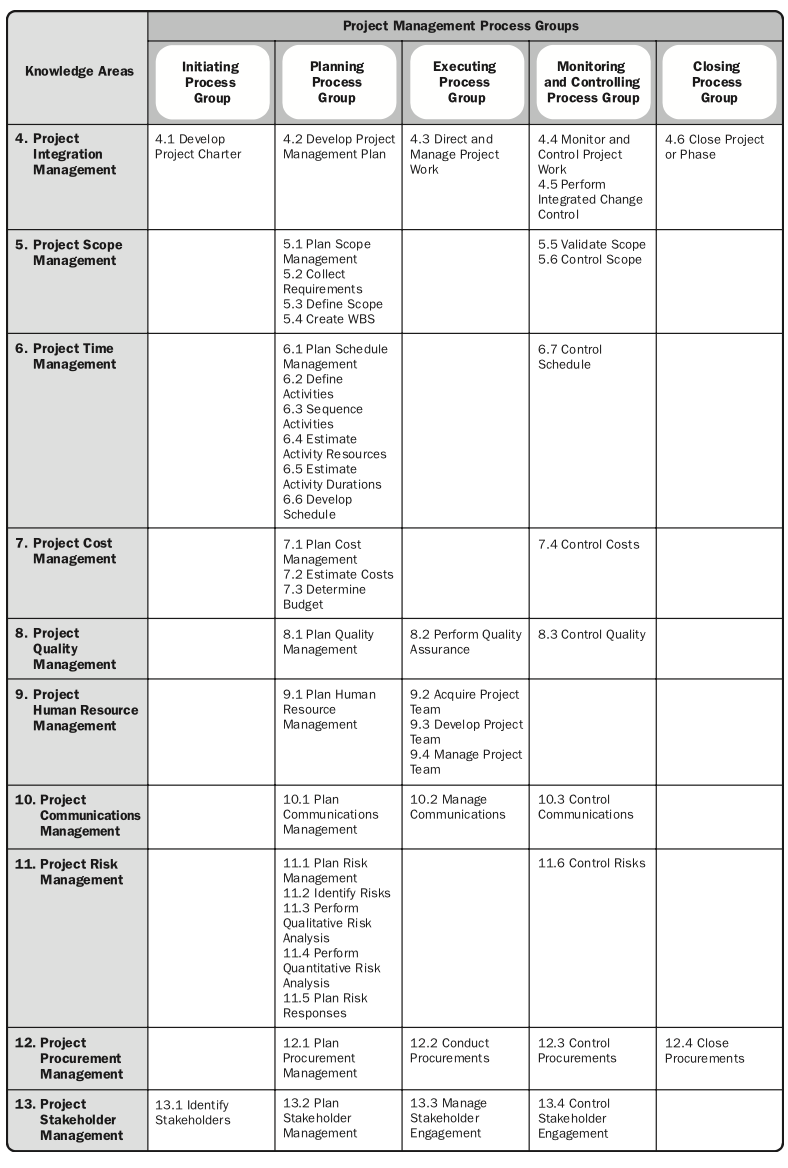
\includegraphics[width=\textwidth]{img/PMBOKprocesses.png}
\caption{PMBOK processes organized by group and area of knowledge. Extracted from \cite{pmbok5}.}
\end{figure}


This guide also provides some background on the project management area, defining common vocabulary and establishing concepts necessary to fully understand all processes. Presents characteristics of projects, programmes and portfolios, roles of project managers and organizational aspects that influence the management process, like organizational structures, culture, assets or stakeholders.\par 
Another important aspect of PMBOK is that is a more general framework, making it necessary to complement with other frameworks or guides when applying to a specific area. This guide only presents the general processes for project management, lacking on implementation details for specific areas, like the area of IT Management.\par 

\subsubsection{PMBOK critical analysis}

The importance of PMBOK for this project is related to its widely acceptance and adoption as the reference guide to project management by many professionals in the area, being tested and evaluated its importance in terms of good practices adopted in project management. Despite being more general and lacking in specificity to IT management, it can be complemented with the two previous frameworks presented (COBIT and ITIL), using some more detailed guidance of ITIL and COBIT to improve PMBOK focus to this project.\par
PMBOK presents processes for all phases of the life cycle of a project, being too extensive considering the theme of this project and the time-frame available. For this scope, we will only be able to consider a subset of all processes presented, being necessary, in the solution's architecture phase of this project, present a mapping between processes covered on PMBOK relating with processes of COBIT and ITIL.


\section{Relevant International Standards}

In this section we will present the international standards that are referenced or important to complement the frameworks previously presented. These standards will allow us to design processes in conformance with practices that are considerer as the reference in some areas of project management.\par
We will analyze the ISO/IEC 12207\cite{ISO12207}, an systems and software engineering international standard for Software life cycle processes. This standard will allow us to define the processes that are important to consider in the scope of this project. It will provide an high-level process reference for the complete life cycle of a software system\par
Relating to COBIT, we have standards that are directly correlated to it, as the ISO/IEC 20000\cite{ISO20000-1,ISO20000-2,ISO20000-3,ISO20000-4,ISO20000-5}, a set of international standards for IT service management, and ISO/IEC 27000\cite{ISO27000}, a set of international standards for information security management systems.\par
For other standards more general to all frameworks we will present the ISO 31000\cite{ISO31000,IEC31010}, a set of standards that provide principles, framework and a process for managing risk, and ISO 19011\cite{ISO19011}, a international standard for providing guidelines for auditing management systems. This standards will complement complex areas of project management providing some additional and specific knowledge.

\subsection{ISO/IEC 12207}

As described by ISO/IEC 12207:2008 \cite{ISO12207}, it \textit{``establishes a common framework for software life cycle processes, with well-defined terminology, that can be referenced by the software industry. It contains processes, activities, and tasks that are to be applied during the acquisition of a software product or service and during the supply, development, operation, maintenance and disposal of software products.''}. The main objective of this standard is to present standardized processes that will make easier the communication among all stakeholders in the software product life cycle.\par
This standard groups the processes to be performed during the life cycle of a software project in seven groups . It presents, for each process, its objectives and expected results as well as the necessary activities to implement it. The processes are grouped in 7 groups, related to the phase they are applied during the software life cycle. All processes are listed in figure 6.

\begin{itemize}
  \item Agreement processes
  \item Organizational Project-Enabling Processes
  \item Project Processes
  \item Technical Processes
  \item Software Implementation Processes
  \item Software Support Processes
  \item Software Reuse Processes 
\end{itemize}

 
\begin{figure}[h!]
\centering
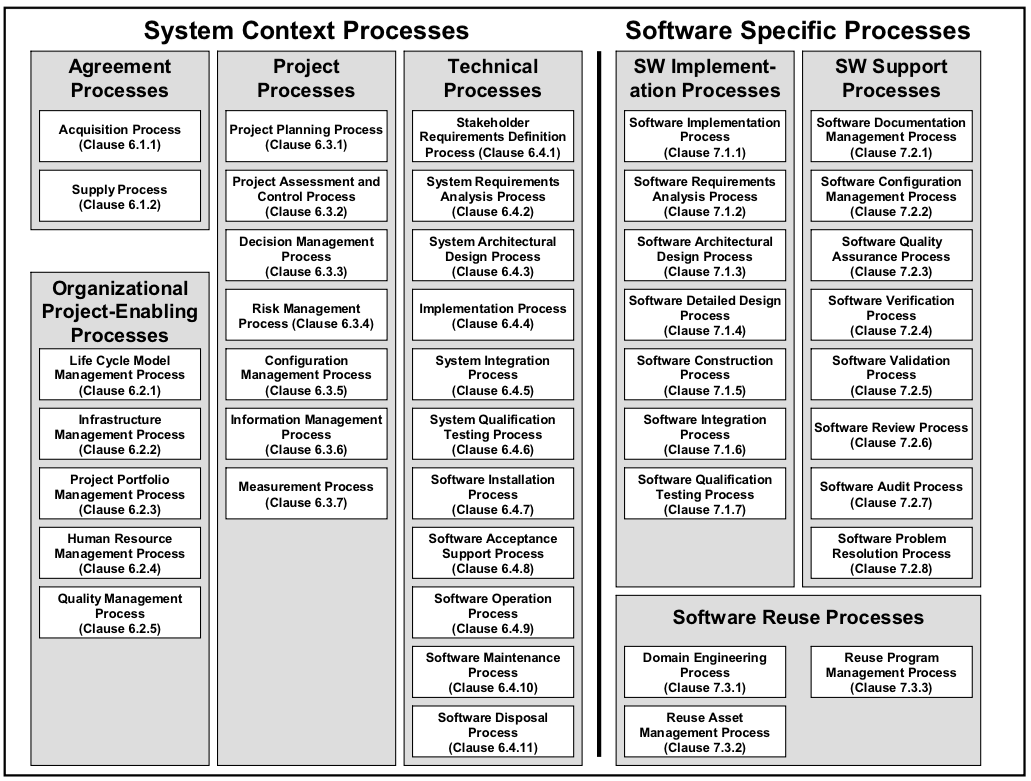
\includegraphics[width=\textwidth]{img/ISO12207Processes.png}
\caption{ISO/IEC 12207 processes. Extracted from \cite{ISO12207}.}
\end{figure}

It may be used standalone or jointly with ISO/IEC 15288\cite{ISO15288}, an international standard for system life cycle processes, and supplies a process reference model that supports process capability assessment in accordance with ISO/IEC 15504\cite{ISO15504}, a set of technical standards documents for the computer software development processes assessment.\par
This standard is important for this project in the way it standardize the processes for the whole life cycle of the software, grouping the processes for a better understanding its scope. We will use this standard, specifically figure 6, to present the processes that make part of the scope of this project, after what we will relate them with the frameworks previously presented. 


\subsection{ISO/IEC 20000}

ISO/IEC 20000 corresponds to a standard on IT Service Management. Initially was developed to reflect best practice guidance contained in some frameworks like ITIL, COBIT or Microsoft operations. This standard in composed by 5 parts:

\begin{itemize}
  \item \textbf{ISO/IEC 20000-1:2011} -  Corresponds to the most relevant part of the ISO/IEC 20000 standard. It specifies requirements for the service provider to manage the whole system life cycle. Similar to the ITIL V3 view, the requirements include the design, transition, delivery and improvement of services to agree with the service requirements established.\cite{ISO20000-1}\par
  
  \vspace{5mm}
  
  \item \textbf{ISO/IEC 20000-2:2012} - Provides guidance on implementing Service management systems defined by the requirements of ISO/IEC 20000-1. As presented by ISO/IEC 20000-2 \cite{ISO20000-2}, \textit{``Enables organizations and individuals to interpret ISO/IEC 20000-1 more accurately, and therefore to use it more effectively. The guidance includes examples and suggestions to enable organizations to interpret and apply ISO/IEC 20000-1, including references to other parts of ISO/IEC 20000 and other relevant standards.''}.\par
  
  \vspace{5mm}
  
  \item \textbf{ISO/IEC 20000-3:2012} - Used by service providers, consultants and assessors, provides guidance on scope definition, applicability and demonstration of conformity to ISO/IEC 20000-1 requirements specification. It also contains assessment standards.\cite{ISO20000-3}\par
  \vspace{5mm}
  
  \item \textbf{ISO/IEC TR 20000-4:2010} - This standard acts as a facilitator for developing a process assessment model according to ISO/IEC 15504 process assessment principles. Related to ISO/IEC 15504, ISO/IEC 15504-1 describes the concepts and terminology used for process assessment and ISO/IEC 15504-2 describes the requirements for the conduct of an assessment and a measurement scale for assessing process capability.\cite{ISO20000-4}\par
  
  \vspace{5mm}
  
  \item \textbf{ISO/IEC TR 20000-5:2013} - This standard presents an implementation plan on how to implement a service management system to fulfill the requirements of ISO/IEC 20000-1:2011. This standard is planned to be used by service providers but can also be used for his advisors to provide guidance on how to implement an service management system.\cite{ISO20000-5}\par
  
  \vspace{5mm}

  This standard is a clear complement to the ITIL framework, providing a similar view for the framework previous presented but being more complete in terms of requirements identification and process assessment. ITIL lacks of a process assessment model and detailed implementation plans, being this standard a way to fulfill those problems.\par
  
\end{itemize}

\subsection{ISO/IEC 27000}

ISO/IEC 27000\cite{ISO27000} is family of international standards related to Information Security management systems (ISMS). This set of standards intent to help organizations of any size to implement and operate an ISMS. As stated by ISO, this family of standards contain information on:

\begin{itemize}

\item Requirements definition for an ISMS and for certification of those systems.
\item Support and guidance for the overall process to establish, implement, maintain and improve and ISMS.
\item Conformity assessment for ISMS.
\item Terms and definitions related to Information security management.

\end{itemize}

This family of standards is commonly used by organizations to implement frameworks for managing information security, protecting important assets as financial data or customers details. Information security is one of the main concerns on any organization, because information leaks or losses can have severe consequences for the overall organization.\par
International standards as ISO 31000 and ISO 19011 are also related to this family of standards, making risk management and auditing management systems, respectively, areas that have direct impact on information security management systems. Dealing with information security is impossible without considering risk. The overall ISMS need to take account processes for risk identification, treatment and assessment for establishing a secure management system. Furthermore, and also related to risk, ISMS need to consider auditing management as a way to ensure information security and its correct management.\par
This standard will be important for our project considering we deal with processes that consume and produce information, and all information is an important asset for any organization implement this processes, making this standard fundamental to establish an information security management system to protect all the information we deal with.\par


\subsection{ISO 31000}

ISO 31000 is a set of standards related to risk management. ISO 31000:2009, Risk management - Principles and guidelines, provides principles, framework and a process for managing risk. It can be used by any organization independently of its context of operation (size, sector, activity). As presented by this standard \cite{ISO31000}, \textit{``Using ISO 31000 can help organizations increase the likelihood of achieving objectives, improve the identification of opportunities and threats and effectively allocate and use resources for risk treatment.''}.\par
In figure 7, we can observe the purposed framework by ISO 31000:2009, used to implement risk management on the management system of the organization. Many organizations have already frameworks for implementing risk management, distinct from ISO 31000, but that can be evaluated and reviewed against this international standard in order to check its suitability. In figure 8 are presented the processes for Risk management implementation.\par

\begin{figure}[h!]
\centering
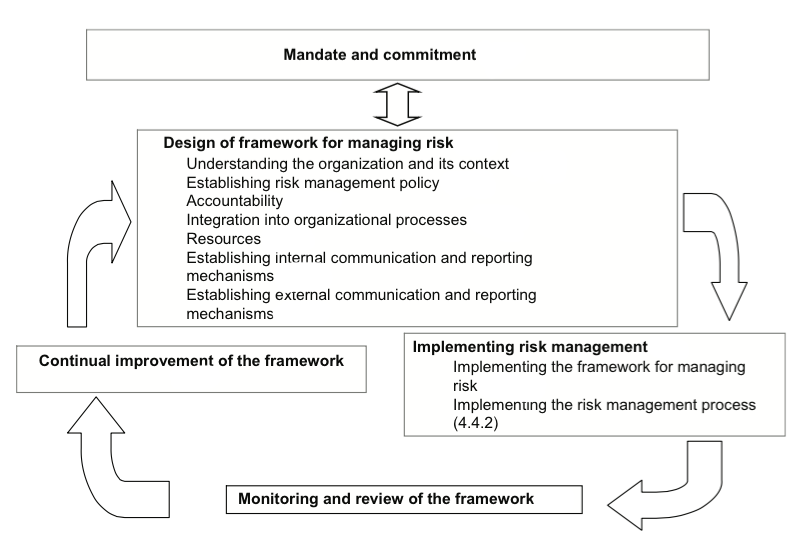
\includegraphics[width=0.6\textwidth]{img/ISO31000Framework.png}
\caption{ISO 31000:2009 framework for Risk Management. Extracted from \cite{ISO31000}.}
\end{figure}

\begin{figure}[h!]
\centering
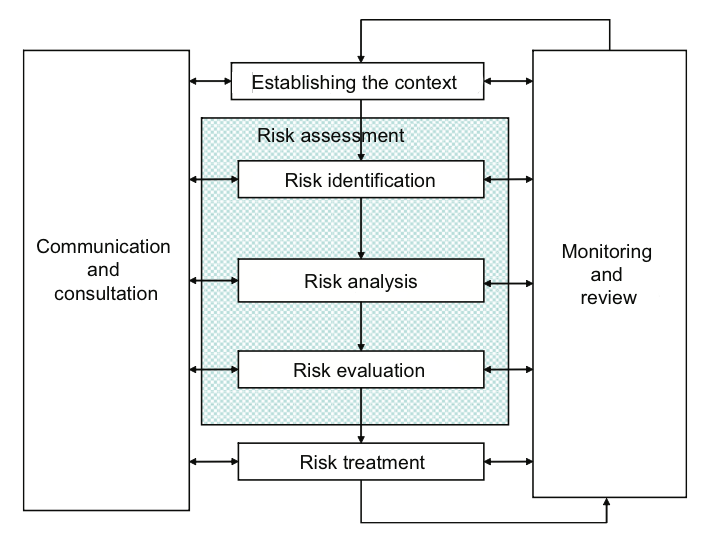
\includegraphics[width=0.6\textwidth]{img/ISO31000RiskProcesses.png}
\caption{ISO 31000:2009 Risk Management Processes. Extracted from \cite{ISO31000}.}
\end{figure}

As confirmed by ISO in this standard, it cannot be used for certification purposes, in the way it doesn't provide guidance for audit programmes, but can be used to compare the risk management processes of the organization with international standard benchmarks.\par
Risk management is a very complex area on project management. It is connected to the whole life cycle of a project and need to be controlled and assessed in many phases and by different forms. IEC 31010:2009, Risk management - Risk assessment techniques focuses on risk assessment. Risk assessment helps organizations understand the risks that could jeopardize the achievement of management and governance goals as well as the suitability of the risk control activities already in place.\cite{IEC31010}\par
The relevance of ISO 31000 for this project focuses on its orientation to an important and complex area of project and maintenance management, providing a framework for Risk management, as well as a set of processes to implement it. It is important to clearly define the scope of this standard related to this project, trying to reduce the complexity and increase its utility for the processes we pretend to design.


\subsection{ISO 19011}

As defined by this International Standard \cite{ISO19011}, \textit{``ISO 19011 provides guidance on auditing management systems, including the principles of auditing, managing an audit programme and conducting management system audits, as well as guidance on the evaluation of competence of individuals involved in the audit process, including the person managing the audit programme, auditors and audit teams. It is applicable to all organizations that need to conduct internal or external audits of management systems or manage an audit programme.''}.\par
In Appendix C it is presented the process flow for the management of an audit programme, described in this international standard. This process can be specially important for our project if we pretend to introduce the auditing processes in the scope of the processes to design. We can use the process flow presented in figure 10 to help designing a auditing process.


\section{A State of the Art in Market Solutions}

Considering we are interested in developing a logical application architecture, we need to analyze solutions available on the market to compose this architecture. This solutions should be evaluated accordingly with its importance and benefit for project purposes, namely for improving our performance in project management and evolving maintenance.\par
Considering this two areas of interest for this project, we will perform an analysis of the solutions available on the market for Project and Portfolio Management Tools (PPM Tools) and for IT Service Support Tools (ITSM Tools). There are hundreds of solutions available for both tools, so we need to find mechanisms for narrowing and evaluating some of the solutions fairly and taking in account its functionalities and benefits for this project. Thus, we will use researches performed in this areas by Gartner and Forrester, two companies focused on IT research and advisory. Both companies provide techniques to evaluate PPM and ITSM tools, providing us the necessary information to evaluate the market offers and perform a usage proposal based on this results.\par

\subsection{Gartner Research}

Gartner inc. is an information technology research and advisory company that delivers to its clients technology-related insight for helping on business decisions. As stated by Gartner \cite{GartnerAbout}, \textit{``From CIOs and senior IT leaders in corporations and government agencies, to business leaders in high-tech and telecom enterprises and professional services firms, to technology investors, we are the valuable partner to clients in over 9,100 distinct enterprises worldwide.''}.\par
Gartner provides a set of methodologies to help clients on its IT investments, reducing and managing risks as well as helping to achieve sucess through research processes that are based in years of experience and maturation. Gartner objective is to provide methodologies that ensure business decisions by clients are made with high levels of confidence.\par
Considering this project objectives, we will use the following methodologies from Gartner:

\subsubsection{Gartner Magic Quadrant}

The objective of the Gartner Magic Quadrant\cite{GartnerMagicQuadrant} is to provide a wide-angle view of the relative positions of a specific market's competitors. It helps on analyzing how well technology providers are executing against their stated vision, presenting a graphical competitive positioning (see figure 9) of four types of technology providers, in growing markets with providers differentiation. The four types of technology providers are:

\begin{itemize}
\item \textbf{Leaders} - Execute well against their current vision and are well positioned for tomorrow.
\item \textbf{Visionaries} - understand where the market is going or have a vision for changing market rules, but do not yet execute well.
\item \textbf{Niche Players} - Focus successfully on a small segment, or are unfocused and do not out-innovate or outperform others.
\item \textbf{Challengers} - Execute well today or may dominate a large segment, but do not demonstrate an understanding of market direction.
\end{itemize}

\begin{figure}
\centering
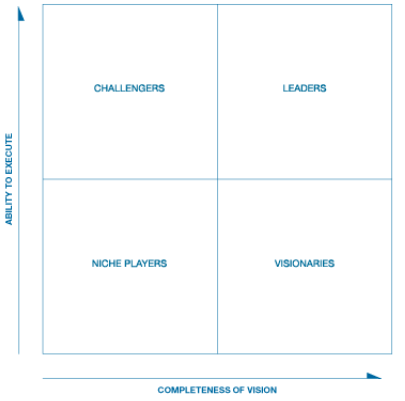
\includegraphics[width=0.4\textwidth]{img/GartnerMagicQuadrant.png}
\caption{Gartner Magic Quadrant representation. Extracted from \cite{GartnerMagicQuadrant}.}
\end{figure}

This methodology is fundamental to analyze technology providers we can consider for adoption, but we need to take in account on how each provider aligns with the business goals of the organization. focusing on the leaders' quadrant is bot always the best option and we need to know what specific objectives we want to achieve to select the best provider for fulfilling our requirements. 


\subsubsection{Gartner MarketScope}

Gartner MarketScope methodology\cite{GartnerMarketScope} is used for analyzing solutions for emerging markets with changing requirements. Gartner Magic Quadrant is not suitable for this type of markets as far as a competitive positioning is not useful and accurate for an growing and changing market. Thus, MarketScope intents to understand how the status of an emerging market aligns with clients state of maturity and future plans. It helps evaluating participating technology providers against the Gartner vision for that market. MarketScopes rate each market's participating technology providers as Strong Positive, Positive, Promising, Caution or Strong Negative.\par

\subsubsection{Gartner Critical Capabilities}

This methodology\cite{GartnerCriticalCapabilities} will complement Gartner Magic Quadrant, providing deeper insight into providers' solutions, presenting its offerings based on service and product key capabilities ratings. As stated by Gartner\cite{GartnerCriticalCapabilities}, \textit{``a Critical Capabilities document is a comparative analysis that scores competing products or services against a set of critical differentiators identified by Gartner. It shows you which products or services are a best fit in various use cases to provide you actionable advice on which products/services you should add to your vendor shortlists for further evaluation.''}.\par
This methodology offers better benefits when applied in line with the Magic Quadrant methodology, providing deeper insight on products and services offerings from providers that Magic Quadrant positioned on the market. When available, we will consider these two methodologies together for evaluating PPM and ITSM solutions.\par

\subsection{Forrester Research} 

Forrester is a research and advisory company providing guidance to professionals in 13 key roles across the business technology, marketing and strategy segments.\cite{ForresterAbout} It presents to its clients research-based services, centering its corporate mission on providing client's adaptable and centered solutions to his needs. As stated by Forrester Role Manifesto, its core values, called 3CIQ, are the Clients, Collaboration, Courage, Integrity and Quality.\par
Considering our objectives for this project, we will consider the Forrester Wave Methodology to analyze the PPM and ITSM solutions available on the market.

\subsubsection{Forrester Wave Methodology}

This methodology\cite{ForresterWave} is provided by Forrester to evaluate providers in software, hardware or service market, presenting the criteria and the weights for this evaluation. This methodology is transparent for the client, being only based in criteria weighting performed by Forrester research professionals. In addition, all the methodology process and participants are presented, making clear how the evaluation was conducted.\par
Each Forrester Wave counts with the participation of four key elements: An analyst, a research associate, a vendor response team and costumer references. Before starting the analysis, the analyst performs a preparation process, researching the evaluation category, identifying the category and the scope, selecting and evaluation methods and creating the research plan and timeline.\par
Consider the evaluation process, it is composed by five milestones: Create evaluation criteria, determine vendors for inclusion, gather evaluation data, create the vendor comparison and publish the report. This milestones ensure a well defined and independent process.\par
We will present, for the PPM an ITSM tools, the corresponding Forrester Wave reports, complementing the Gartner evaluation by making our research for this tools more valuable and rich.\par 

\subsection{Project and Portfolio Management Tools analysis}

To perform our analysis on available market solutions for Project and Portfolio Management tools we will use the Gartner Magic Quadrant for IT Project and Portfolio Management from June 2010 \cite{magicQuadrantPPM}, the last published Magic Quadrant for this type of tools. For completing our analysis, we will also present the Gartner MarketScope for IT Project and Portfolio Management Software Applications \cite{MarketScopePPM} and the Forrester Wave Project/Program Portfolio Management from Q4 2012.\cite{forresterWavePPM}\par 

\subsubsection{Gartner Magic Quadrant for IT Project and Portfolio Management (June 2010)}

This Magic Quadrant was the last one published in this area by Gartner, due to the innovations and new requirements for Cloud-based solutions presented in Gartner Magic Quadrant for Cloud-Based IT Project and Portfolio Management Services\cite{magicQuadrantCloud}.
This quadrant focuses on the PPM market, where Gartner defines the core functionalities each PPM tool supplier must take in account to conform with the market needs. This functionalities are the following:

\begin{itemize}
\item \textbf{IT PPM} - Support to Internal IT Project and Portfolio Management.
\item \textbf{NPD} - New Product Development.
\item \textbf{PSA} - Professional Services Administration.
\item \textbf{AEC} - Traditional architecture, engineering and construction (AEC) environments.
\item \textbf{ITPC} - IT Planning and Control.
\item \textbf{APM} - Application Portfolio Management.
\item \textbf{EPPM} - Enterprise PPM.
\end{itemize}

The Magic Quadrant document\cite{magicQuadrantPPM} also provides some insight on the main challenges and problems the area faces actually and some advices, considerations and definitions for professionals in the area. Considering our purposes, in figure 10 we have the Magic Quadrant for IT Project and Portfolio Management from June 2010, and in figure 11 and 12 we have the Ability to execute and Completeness of vision evaluation criteria, respectively, presenting the weightings used on the evaluation of each supplier.\par

\begin{figure}[h!]
\centering
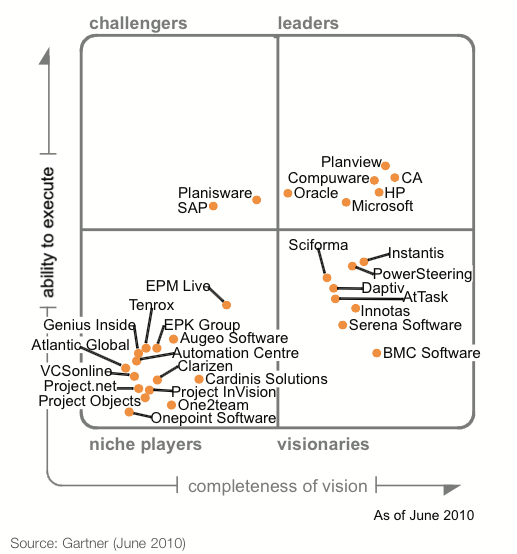
\includegraphics[width=0.6\textwidth]{img/MQPPMTools.png}
\caption{Gartner Magic Quadrant for IT Project and Portfolio Management (June 2010). Extracted from \cite{magicQuadrantPPM}.}
\end{figure}


\begin{figure}[h!]
\begin{minipage}[h!]{0.45\linewidth}
\centering
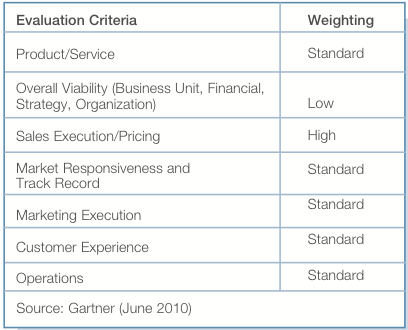
\includegraphics[width=\textwidth]{img/MQPPMToolsAbilityExecute.png}
\caption{Ability to execute evaluation criteria. Extracted from \cite{magicQuadrantPPM}.} 
\label{fig:figure1}
\end{minipage}
\hspace{0.5cm}
\begin{minipage}[h!]{0.45\linewidth}
\centering
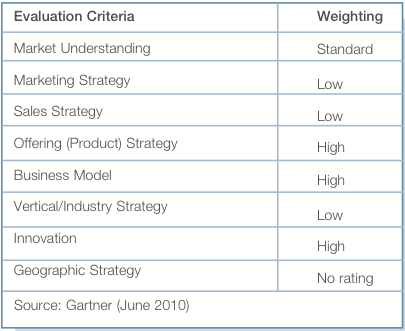
\includegraphics[width=\textwidth]{img/MQPPMToolsCompletess.png}
\caption{Completeness of vision evaluation criteria. Extracted from \cite{magicQuadrantPPM}.}
\label{fig:figure2}
\end{minipage}
\end{figure}



For this magic quadrant, based on our project objectives, we will consider only the quadrant for the leaders taking in account we are looking for the most complete solution on all PPM market areas. For the leaders quadrant, we have product depth in the whole PPM core areas like demand management and analysis, advanced scheduling, resource and cost management and portfolio analysis, establishing a big difference to the challengers quadrant, where only some of them are fully addressed.\par
Leaders also offer different multiple deployment options, as staged implementations, hosted or SaaS, making its solutions more flexible and applicable to different organization realities. Leaders share many attributes with visionaries or challengers, but they establish differentiation with high ratings in many areas.\par
The leaders quadrant is composed by Planview with the product Planview Enterprise, Compuware with ChangePoint, CA with CA Clarity EPM, HP with HP PPM Center, Microsoft with EPM and Oracle with Primavera. In \cite{magicQuadrantPPM} we present the main strengths and cautions for each one of this solutions, based on Gartner's analysis.


\subsubsection{Gartner MarketScope for IT Project and Portfolio Management Software Applications}

This marketScope includes on-premises and cloud-hosted IT project portfolio management (PPM) providers that offers solutions for deploying its IT PPM applications on-site at the customer's facility (on-premises) or in a SaaS (cloud-hosted). This market is constantly growing and providers are investing more on SaaS solutions.\par
As explained by Gartner in \cite{MarketScopePPM} \textit{``On-premises and cloud-hosted IT PPM providers offer deployment options, allowing their customers to deploy a dedicated instance of their IT PPM applications on-site at the customer's facility or in the cloud in a hosting environment offered by the provider as a service''}.\par
For larger organizations, IT PPM solutions are being migrated to SaaS solutions, either for choosing providers presented on this marketScope or by providers presented in the Gartner's ``Magic Quadrant for Cloud- Based Project and Portfolio Management Services."\cite{magicQuadrantCloud}.\par
In this marketScope we have small, midsize and large providers offering on-premises and/or cloud-hosted PPM applications and they are evaluated considering their ability to support large-enterprise IT departments. Consequently, providers with strong positive and positive ratings are suitable for supporting very large to large deployments and some of the ones rated as strong and promising are more suitable for midsize organizations.\par
In table 1 we can see the evaluation criteria for this research, as well as the weights for each criteria. A more detailed evaluation criteria can be consulted in \cite{MarketScopePPM}. In figure 13 is presented the marketScope for IT Project and Portfolio Management Software Applications. An analysis for each product/service in available in the MarketScope document \cite{MarketScopePPM}.
Considering the MarketScope results presented, we can see that the solutions considered for analysis in the Gartner Magic Quadrant obtained a positive or strong positive rating in the MarketScope research. We can conclude this providers, despite being leaders in the PPM market, also provide products/services that are flexible and adaptable to emerging markets with constant changes in requirements.


\begin{table}[h!]
\centering
\begin{tabular}{|c|c|}
\hline
\textbf{Evaluation Criteria} & \textbf{Weighting} \\ \hline
Customer Experience & High \\ \hline
Offering (Product) Strategy & Standard \\ \hline
Product Service & High \\ \hline
Business Model & High \\ \hline
Innovation & High \\ \hline
Market Understanding & High \\ \hline
Market Responsiveness and Track Record & High \\ \hline
\end{tabular}
\vspace{2mm}
\caption{Gartner MarketScope for IT Project and Portfolio Management Software Applications Evaluation Criteria. Adapted from \cite{MarketScopePPM}.}
\label{my-label}
\end{table}

\begin{figure}[h!]
\centering
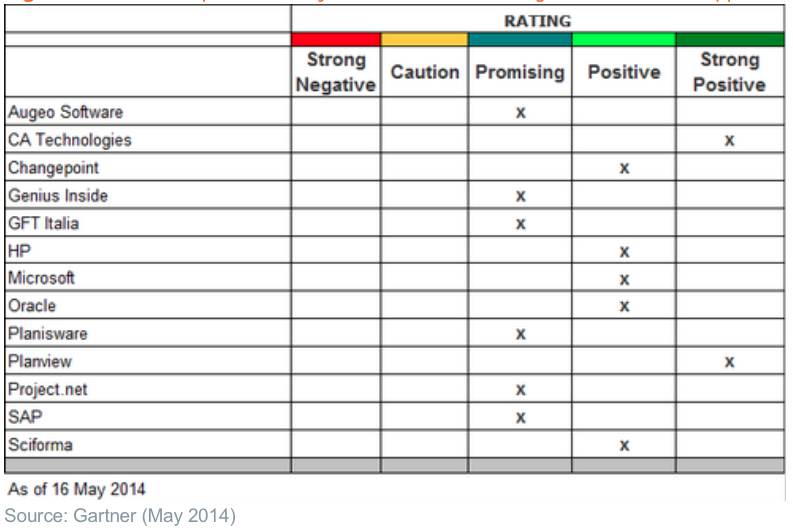
\includegraphics[width=0.6\textwidth]{img/MarketScopePPM.png}
\caption{Gartner MarketScope for IT Project and Portfolio Management Software Applications Results. Extracted from \cite{MarketScopePPM}.}
\end{figure}


\subsubsection{The Forrester Wave: Project/Program Portfolio Management, Q4 2012}

As stated by Forrester \cite{forresterWavePPM}, \textit{``Agile development disrupts operations and governance processes such as project/program portfolio management (PPM). That disruption drives a bifurcation in the tools market \- Traditional PPM doesn't suit the lighter-weight/lean governance processes that Agile projects require.''}. Considering this bifurcation, Forrester performed a 68-criteria evaluation of PPM vendors identifying the 10 most significant ones, comparing them  considering market's bifurcation and its constantly change.\par
This research was performed considering two Forrester Wave Models. As defined by Forrester in \cite{forresterWavePPM}, \textit{``Above-the-line vendors serve enterprises primarily interested in portfolio planning, with linkage to tactical work planning and execution. Below-the-line vendors support enterprises seeking immediate help with planning, execution, and work management.''}.\par
The vendors 68-evaluation criteria are grouped in three high-level groups: Current offering (deployment options, global support, and features for top-down portfolio planning or work-driven execution.), Strategy (product strategy, deployment options, support, and pricing) and Market Presence (revenue growth, financial strength, sales and support services, and the ability to support global implementations).\par
The 10 vendors were selected following the vendor selection criteria presented in figure 14. Information about the products offered by this vendors are available in figure 15.\par


\begin{figure}[h!]
\begin{minipage}[h!]{0.45\linewidth}
\centering
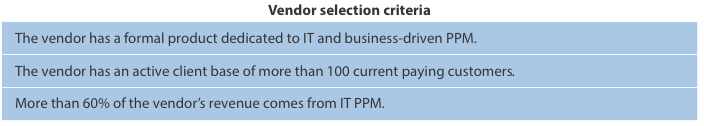
\includegraphics[width=\textwidth]{img/AboveLineCriteria.png}
\caption{Vendors selection criteria. Extracted from \cite{forresterWavePPM}.}
\label{fig:figure1}
\end{minipage}
\hspace{0.5cm}
\begin{minipage}[h!]{0.55\linewidth}
\centering
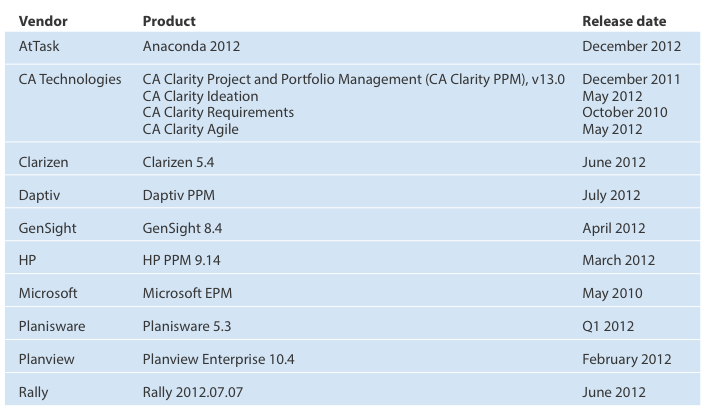
\includegraphics[width=\textwidth]{img/AboveLineVendors.png}
\caption{Above the line selected vendors. Extracted from \cite{forresterWavePPM}.}
\label{fig:figure2}
\end{minipage}
\end{figure}

In figure 16 we can see the Forrester Wave for Above-The-Line Project/Program Portfolio Management and in figure 17 the detailed scores by high-level criteria. HP, CA Technologies, Planview, and Daptiv are leaders for this market, being followed by Microsoft, Planisware, Rally, AtTask, and Clarizen that offers competitive solutions, with less strategic alignment capabilities than the leaders group. GenSight has good and solid functionalities, some of them exceeding the leaders ones, but takes a much specialized approach for portfolio management, obtaining a very low score on strategy criteria.\par
Considering the leaders group, HP's strategy for integrated portfolio management and delivery makes it a Leader while CA Technologies offers robust analytics at transactional and strategic levels. Analytics and integration are the best qualities for Planview and Daptiv's functional strength on multiple fronts makes it stand out.\par


\begin{figure}[h!]
\begin{minipage}[h!]{0.40\linewidth}
\centering
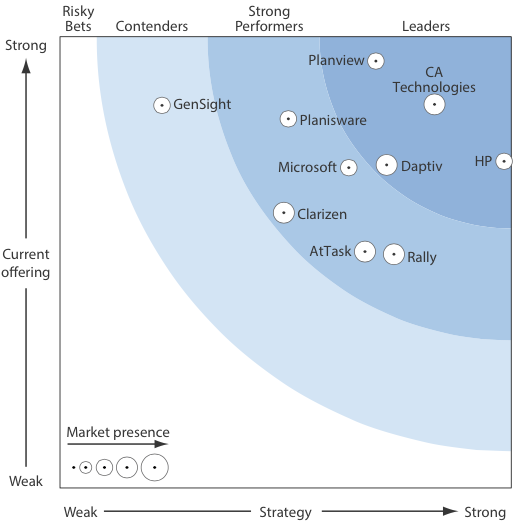
\includegraphics[width=\textwidth]{img/AboveLineWave.png}
\caption{Forrester Wave for Above-The-Line Project/Program Portfolio Management. Extracted from \cite{forresterWavePPM}.}
\label{fig:figure1}
\end{minipage}
\hspace{0.5cm}
\begin{minipage}[h!]{0.60\linewidth}
\centering
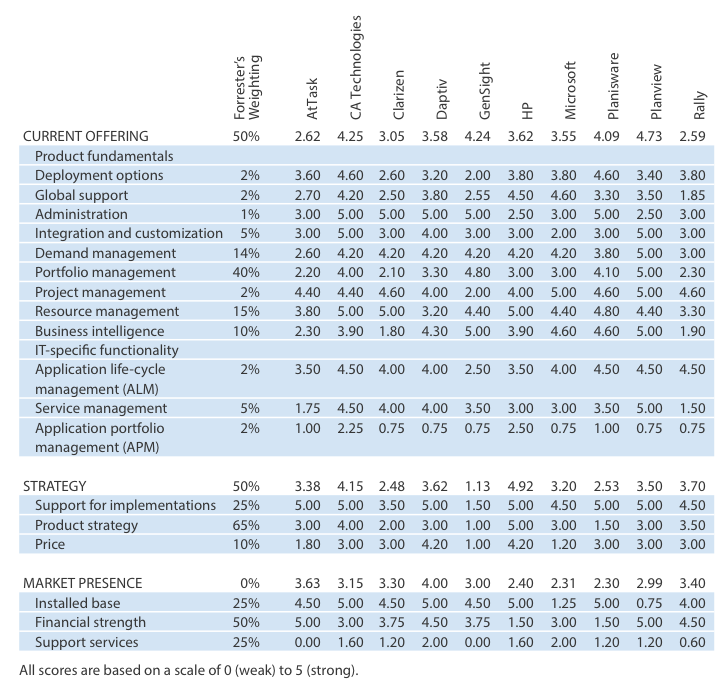
\includegraphics[width=\textwidth]{img/AboveLineScores.png}
\caption{Forrester Wave for Above-The-Line Project/Program Portfolio Management detailed scores by high-level criteria. Extracted from \cite{forresterWavePPM}.}
\label{fig:figure2}
\end{minipage}
\end{figure}



In figure 18 we can see the Forrester Wave for Below-The-Line Project/Program Portfolio Management and in figure 19 the detailed scores by high-level criteria. HP, Planview, and CA Technologies are clearly the big leaders, proving good features on Agile planning, resource management and reporting support. Microsoft, Rally, and Daptiv are also leaders, but with lower scores on current offering and strategy criteria groups. AtTask, Clarizen, and Planisware offer competitive solutions facing leaders solutions, but are designed for different types of work environments. GenSight solution is too much strategic planning oriented, making it only a contender for leaders and strong performers\par
Considering the leaders group, HP Project Management provides the best solution in terms of managing various types of projects from traditional to Agile. Planview places its emphasis on pipeline management, resource planning, and reporting. CA Clarity PPM provides the most comprehensive planning solutions for project and work management while Microsoft EPM is the best project-planning tool at the desktop level. Rally has an outstanding performance as agile project management tool. Daptiv provides interesting functionalities on project and work management.\par

\begin{figure}[th!]
\begin{minipage}[th!]{0.40\linewidth}
\centering
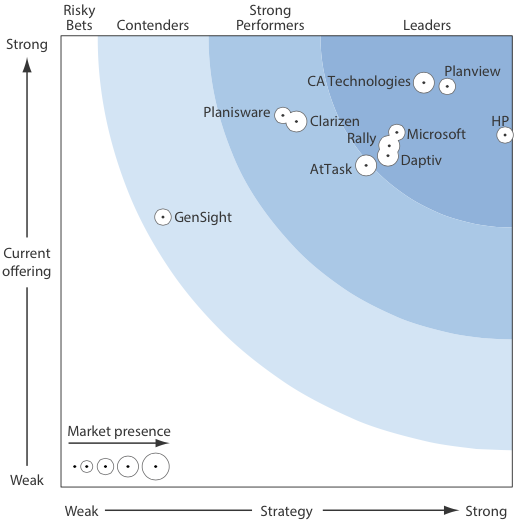
\includegraphics[width=\textwidth]{img/BelowLineWave.png}
\caption{Forrester Wave for Below-The-Line Project/Program Portfolio Management. Extracted from \cite{forresterWavePPM}.}
\label{fig:figure1}
\end{minipage}
\hspace{0.5cm}
\begin{minipage}[th!]{0.60\linewidth}
\centering
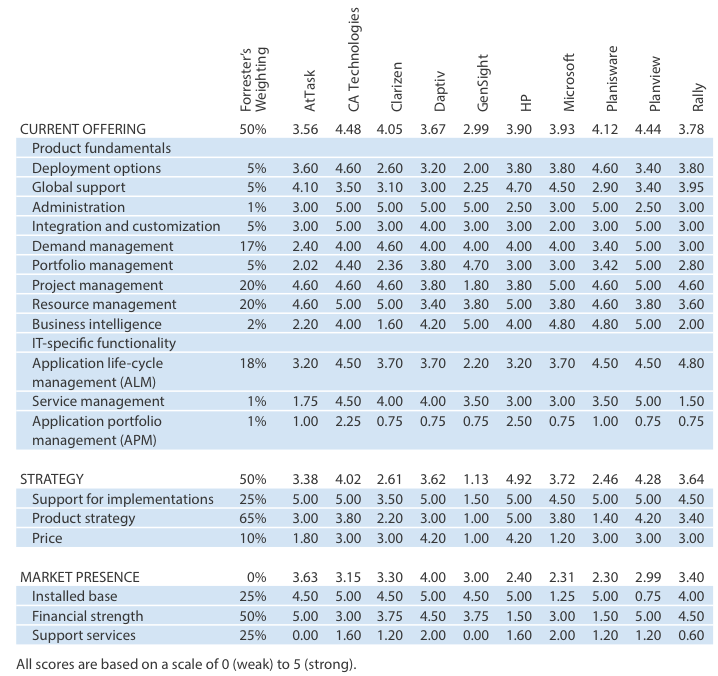
\includegraphics[width=\textwidth]{img/BelowLineScores.png}
\caption{Forrester Wave for Below-The-Line Project/Program Portfolio Management detailed scores by high-level criteria. Extracted from \cite{forresterWavePPM}.}
\label{fig:figure2}
\end{minipage}
\end{figure}

\subsection{IT Service Support Management Tools analysis}

To assess the available market solutions for IT Service Support Management tools we will use the Gartner Magic Quadrant for IT Service Support Management Tools from August 2014\cite{magicQuadrantITSM}. Also from Gartner, we will analyze the Critical Capabilities for IT Service Support Management Tools from August 2014\cite{criticalCapabilitiesITSM}. To provide a more wider and heterogeneous view for this type of tools, we will consider the Forrester Wave: ITSM SaaS Delivery Capabilities, Q3 2014\cite{forresterWaveITSM}\par 

\subsubsection{Magic Quadrant for IT Service Support Management Tools}

This Magic Quadrant provides a precious support on ITSM tools analysis for professionals in IT Service Management. ITSSM tools help on management processes of IT services delivered by the organization, automatizing the tasks and workflows for quality IT services delivery to the business.\par
As stated by Gartner in \cite{magicQuadrantITSM}, \textit{``the market for ITSSM tools is segmented according to the vendors' abilities to provide strong ITSSM capabilities and high levels of ease of integration with broader IT operations management functionalities.''}. Therefore, we can have basic, intermediate and advance vendors considering its ability to integrate with third-party IT Operations Management solutions and the set of ITSM functionalities. Each organization should analyze its own Infrastructure and Operations (I\&O) maturity level and choose an adequate solution. Basic or intermediate vendors are suitable for low maturity I\&O organizations while advance vendors are better option for the high maturity ones.\par
In figure 20 we have the Magic Quadrant for IT Service Support Management Tools from August 2014, and in figure 21 and 22 we have the Ability to execute and Completeness of vision evaluation criteria, respectively, presenting the weightings used on the evaluation of each supplier.\par

\begin{figure}[h!]
\centering
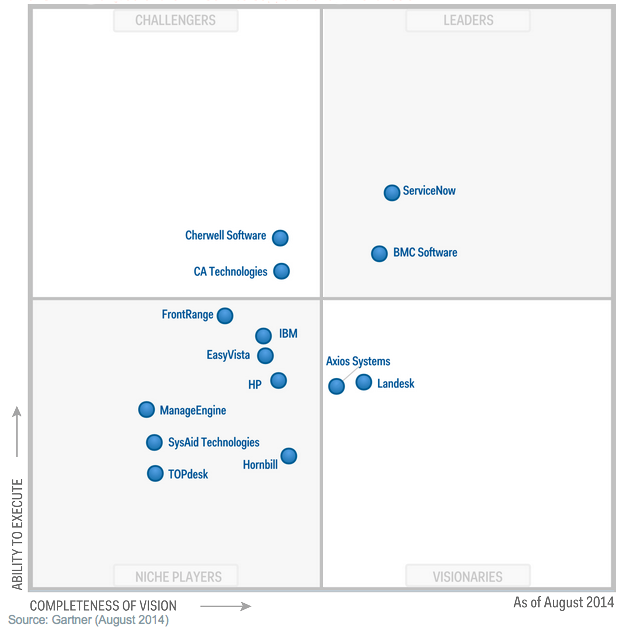
\includegraphics[width=0.6\textwidth]{img/GartnerITSMQuadrant.png}
\caption{Gartner Magic Quadrant for IT Service Support Management Tools (August 2014). Extracted from \cite{magicQuadrantITSM}.}
\end{figure}

\begin{figure}[h!]
\begin{minipage}[h]{0.45\linewidth}
\centering
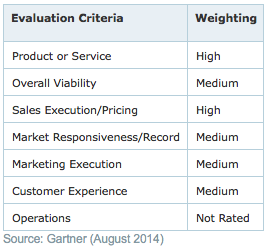
\includegraphics[width=0.8\textwidth]{img/AbilityToExecuteITSM.png}
\caption{Ability to execute evaluation criteria. Extracted from \cite{magicQuadrantITSM}.}
\label{fig:figure1}
\end{minipage}
\hspace{0.5cm}
\begin{minipage}[h!]{0.45\linewidth}
\centering
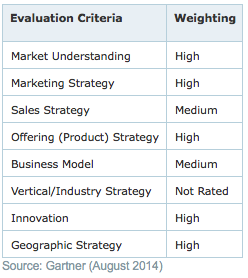
\includegraphics[width=0.8\textwidth]{img/CompletenessOfVisionITSM.png}
\caption{Completeness of vision evaluation criteria. Extracted from \cite{magicQuadrantITSM}.}
\label{fig:figure2}
\end{minipage}
\end{figure}


For this magic quadrant, and considering our project objectives, we will consider only the Leaders and Challengers quadrants, taking in account we are interested in a complete ITSM solution suited for different levels of maturity on I\&O management. For the leaders quadrant, composed by BMC and ServiceNow, we have good market shares (29\% and 21\% respectively) and the desired levels of marketing and sales capabilities for market acceptance.\par 
In the challengers quadrant, CA Technologies and Cherwell Software have growing shares of the market and present good improvements for products providing ITSM solutions. They offer its competitive products with good viability levels for the market.\par
Considering the results presented in this magic quadrant, we will consider the following solutions: ServiceNow IT Service Automation Suite from ServiceNow, BMC Remedy ITSM Suite, BMC FootPrints Service Core and BMC Remedyforce from BMC Software, Cherwell Service Management from Cherwell Software and CA Service Management and CA Cloud Service Management from CA Technologies.\par

\subsubsection{Gartner Critical Capabilities for IT Service Support Management Tools}

For complementing the vendors analysis performed by the Gartner Magic Quadrant for IT Service Support Management Tools, we will also consider the Gartner's Critical Capabilities for IT Service Support Management Tools from August 2014\cite{criticalCapabilitiesITSM}, providing an evaluation of ITSSM tools' critical capabilities in five use cases.\par
As defined by Gartner in \cite{criticalCapabilitiesITSM}, the use cases evaluated are:

\begin{itemize}
\item \textbf{Low to Medium Maturity} - Focused on incident and problem management capabilities, high ease-of-use levels, and out-of-the-box best-practice capabilities.
\item \textbf{Medium to High Maturity} - Focused on incident and problem management capabilities, with increased weighting for integrated change, configuration and release management capabilities.
\item \textbf{High Maturity} - Places significant weight on change, configuration and release capabilities, as well as integration with broader ITOM functionalities.
\item \textbf{Digital Workplace} - Focuses on high weights for IT service request management and IT knowledge management. This scores the products' ability to appeal to business users.
\item \textbf{Total ITSSM} - Organizations focus on a single tool or suite of tools from one vendor to provide broad service support management functions.
\end{itemize}

For product capabilities ratings, Gartner uses the following capabilities:

\begin{itemize}
\item Incident and Problem
\item Change, Configuration and Release
\item Service Request Management
\item IT Knowledge Management
\item Reporting and Dashboards
\item Out-of-the-Box Best Practices
\item Data Source/ITOM Tool Integration
\item Telephony/UCC Platform Integration
\item Product Setup and Complexity
\end{itemize}

From figure 23 to figure 27 we have the products or services score for each use case considered. As we can see, for Low to Medium Maturity use case, Cherwell and EasyVista solutions are the one that have the higher score, presenting good incident and problem management capabilities, high ease-of-use levels, and out-of-the-box best-practice capabilities. For the all other use cases, ServiceNow and BMC solutions lead the market, providing good scores for all the desired capabilities on an ITSM tool.\par
More detailed information on each product or service performance on this evaluation can be consulted in \cite{GartnerCriticalCapabilities}.


\begin{figure}[!h]
\begin{minipage}[!htb]{0.42\linewidth}
\centering
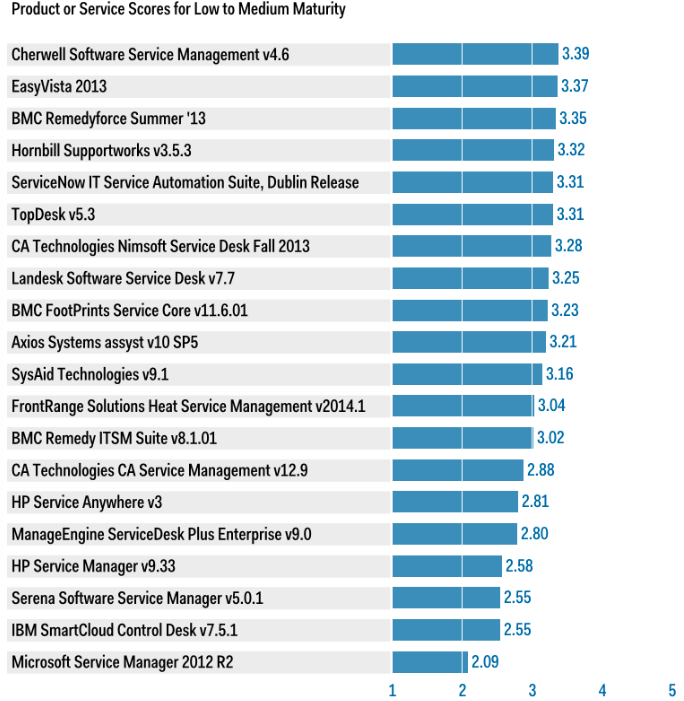
\includegraphics[width=\textwidth]{img/LowMediumScores.png}
\caption{Vendors' Product Scores for the Low to Medium-Maturity Use Case. Extracted from \cite{criticalCapabilitiesITSM}.}
\label{fig:figure1}
\end{minipage}
\hspace{0.5cm}
\begin{minipage}[!h]{0.42\linewidth}
\centering
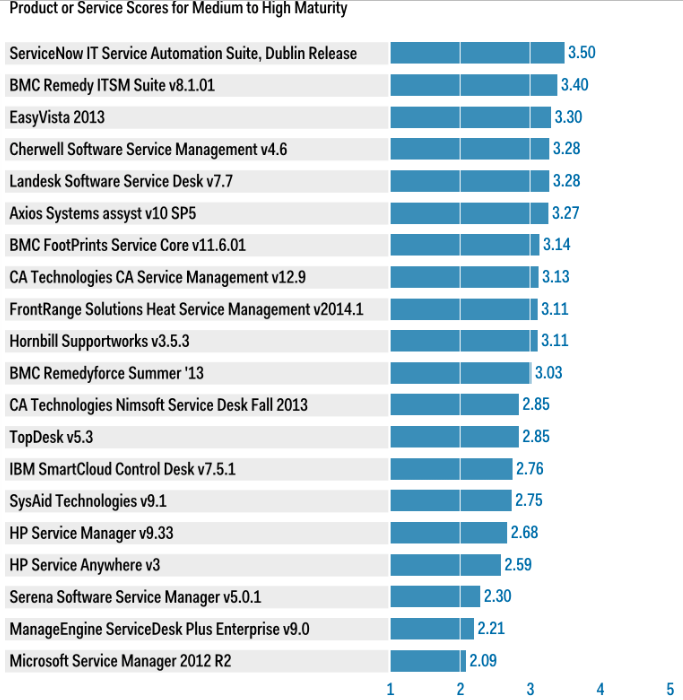
\includegraphics[width=\textwidth]{img/MediumHighScores.png}
\caption{Vendors' Product Scores for the Medium to High-Maturity Use Case. Extracted from \cite{criticalCapabilitiesITSM}.}
\label{fig:figure2}
\end{minipage}
\end{figure}

\begin{figure}[!h]
\begin{minipage}[h]{0.42\linewidth}
\centering
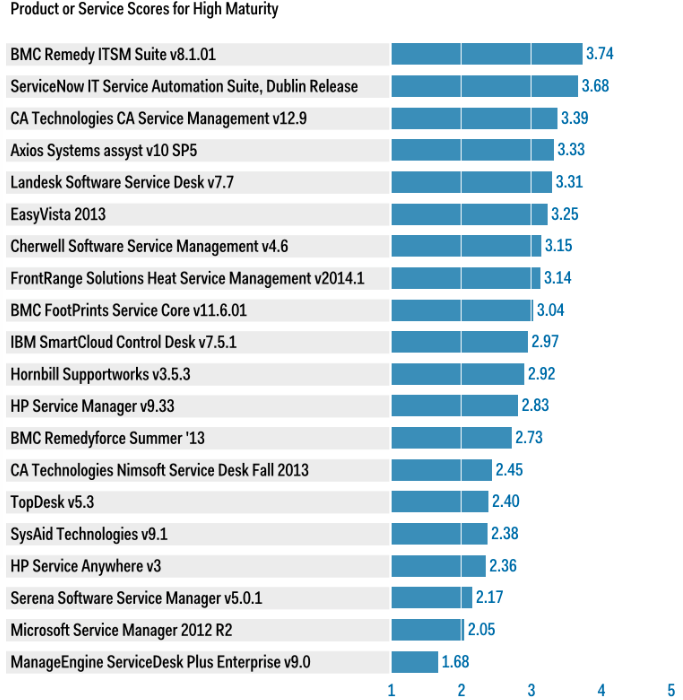
\includegraphics[width=\textwidth]{img/HighScores.png}
\caption{Vendors' Product Scores for the High-Maturity Use Case. Extracted from \cite{criticalCapabilitiesITSM}.}
\label{fig:figure1}
\end{minipage}
\hspace{0.5cm}
\begin{minipage}[!h]{0.42\linewidth}
\centering
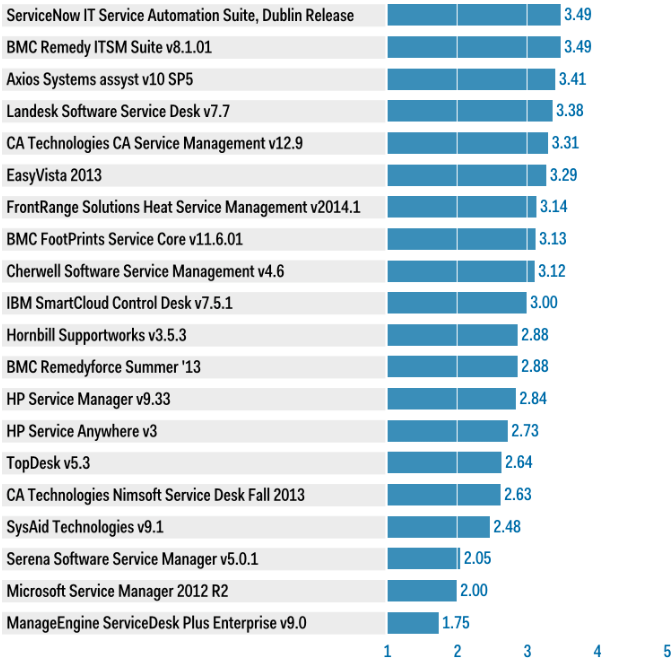
\includegraphics[width=\textwidth]{img/DigitalWorkplaceScores.png}
\caption{Vendors' Product Scores for the Digital Workplace Use Case. Extracted from \cite{criticalCapabilitiesITSM}.}
\label{fig:figure2}
\end{minipage}
\end{figure}


\begin{figure}[!h]
\centering
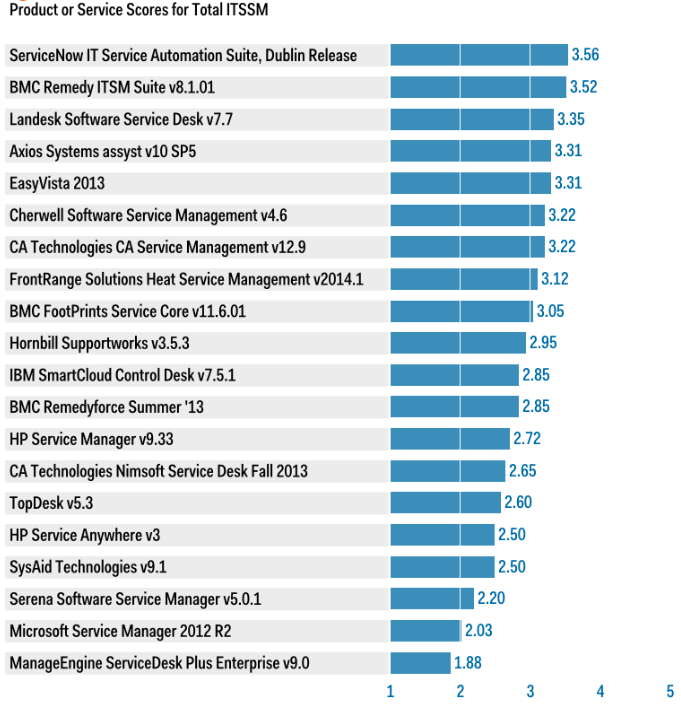
\includegraphics[width=0.40\textwidth]{img/TotalITSMScores.png}
\caption{Vendors' Product Scores for the Total ITSSM Use Case. Extracted from \cite{criticalCapabilitiesITSM}.}
\end{figure}


\subsubsection{Forrester Wave: ITSM SaaS Delivery Capabilities for Q3 2014}

As stated by Forrester in \cite{forresterWaveITSM}, \textit{``How an IT or business service is delivered directly affects the quality of experience for the service consumer and the reputation of the infrastructure and operations (I\&O) team that delivers the services.''}. The need for Saas ITSM vendors' solutions evaluation lead to this 30-criteria Forrester evaluation of the top 10 most significant vendors in ITSM market.\par

The vendors 30-evaluation criteria are grouped in three high-level groups: Current offering (client feedback, scope of predefined service, breadth of offering, availability and resiliency, security and compliance, upgradability and services activation time), Strategy (customer experience, digital disruption, big data and mobile mind shift) and Market Presence (number of enterprise customers, corporate profitability and ITSM SaaS growth).\par
Considering the features and functionality assessment of ITSM SaaS Vendors, the main core areas are: enabling of the most commonly adopted ITSM capabilities (incident, service request, problem, change, knowledge, service-level, and configuration management), the configuration management database (CMDB) or better service information system (SIS), a service portal (or exchange) with self-service capabilities and enabling of social, mobility, and automation capabilities.\par
For this evaluation were considered 10 vendors, selected following the vendor selection criteria presented in figure 28. Information about the products offered by this vendors are available in figure 29.\par

\begin{figure}[h!]
\centering
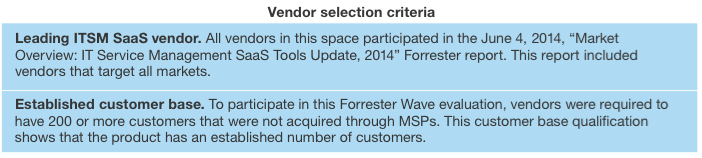
\includegraphics[width=0.7\textwidth]{img/VendorSelectionCriteriaITSM.png}
\caption{Vendors selection criteria. Extracted from \cite{forresterWaveITSM}.}
\end{figure}


\begin{figure}[h!]
\centering
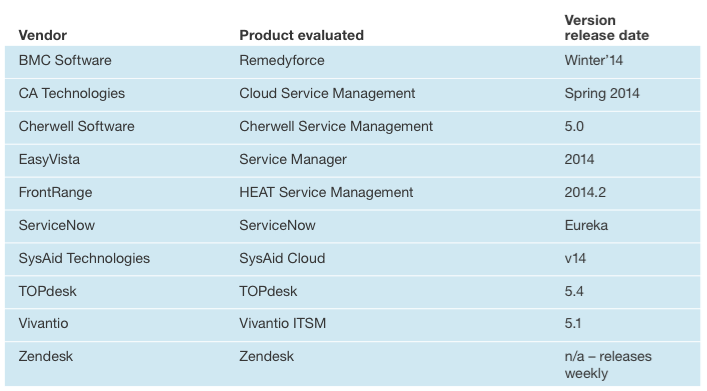
\includegraphics[width=0.7\textwidth]{img/ITSMVendorsInfo.png}
\caption{Top 10 selected vendors. Extracted from \cite{forresterWaveITSM}.}
\end{figure}

In figure 30 we can see the Forrester Wave: ITSM SaaS Delivery Capabilities for Q3 2014 and in figure 31 the detailed scores by high-level criteria. SysAid Technologies, Cherwell Software and ServiceNow are leaders for this market while all the other vendors follows them, being rated as strong performers. The leaders show high ITSM SaaS delivery capabilities and stand apart in customer feedback. While the strong performers vendors present good results for some criteria, they lack on other ones, making them a less complete solution for the ITSM Market\par
All the leaders supply solutions are aimed for all markets, making the difference stand only on specific features or details of each solution. Customers should conduct a detailed analysis to the detailed scores in figure 30 to conclude what is the best solution for a given criteria type.\par


\begin{figure}[h]
\begin{minipage}[h]{0.40\linewidth}
\centering
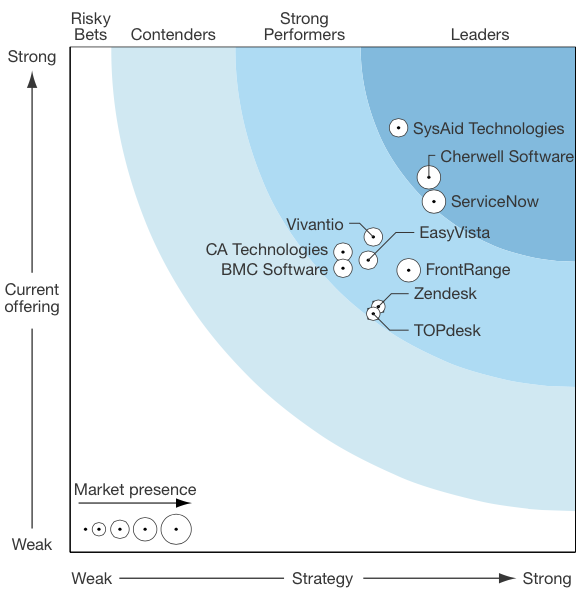
\includegraphics[width=\textwidth]{img/ForresterWaveITSM.png}
\caption{Forrester Wave: ITSM SaaS Delivery Capabilities. Extracted from \cite{forresterWaveITSM}.}
\label{fig:figure1}
\end{minipage}
\hspace{0.5cm}
\begin{minipage}[h]{0.60\linewidth}
\centering
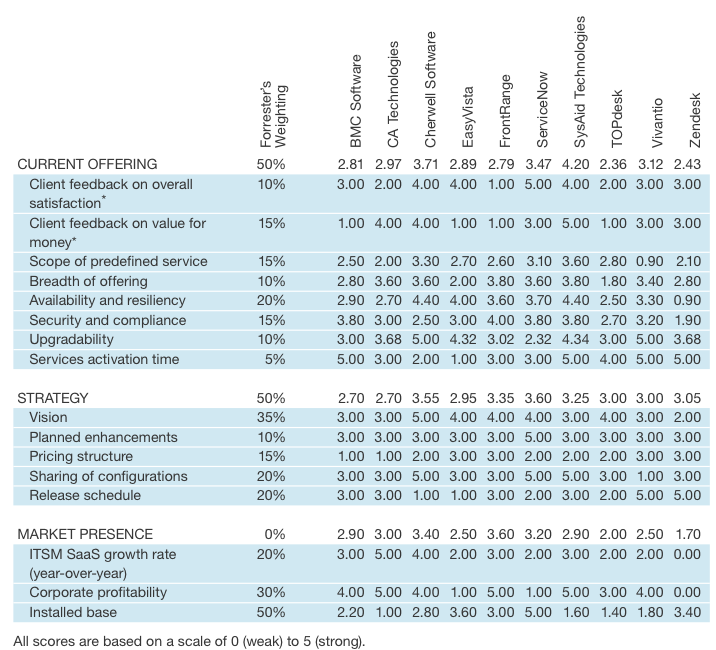
\includegraphics[width=\textwidth]{img/ITSMForrScores.png}
\caption{Forrester Wave: ITSM SaaS Delivery Capabilities detailed scores by high-level criteria. Extracted from \cite{forresterWaveITSM}.}
\label{fig:figure2}
\end{minipage}
\end{figure}

